\part{Introduction to Deep Learning}


\section{Prerequisites}

A student enrolled in this course should have the following skills.

\textbf{Required}:

\begin{itemize}
    \item Working knowledge of derivatives
    \item Knowledge in understanding the key relevant topics of \href{https://www.udacity.com/course/linear-algebra-refresher-course--ud953}{\textbf{Linear Algebra}}:

\begin{itemize}
        \item Vectors, Vector dot and cross products
        \item Inverse functions and transformations: Matrix transformations
        \item Finding inverses and determinants
        \item Matrix multiplication
\end{itemize}

    \item Intermediate Python skills

\begin{itemize}
        \item Represent data using Python's data types: integers, floats, booleans, strings, lists, tuples, sets, dictionaries, compound data structures
        \item Perform data manipulation with Numpy and Pandas
        \item Perform computations and create logical statements using Python’s operators: Arithmetic, Assignment, Comparison, Logical, Membership, Identity
        \item Write conditional expressions using \verb|if| statements and boolean expressions to add decision making to your Python programs
        \item Write user-defined functions / use built-in functions in a library
        \item Produce plots using Matplotlib
        \item Use iterators and generators to create streams of data
        \item Write iteration using \verb|for| statement and indefinite iteration using \verb|while| statements in your Python programs
\end{itemize}

    \item Experience with Jupyter Notebooks
    \item Basic knowledge of machine learning (e.g. Scikit-learn)
\end{itemize}

\textbf{Helpful, but not required}:

\begin{itemize}
    \item Multivariable Calculus
    \item Experience with Anaconda
\end{itemize}

\subsection{Who Should Take This Course}

This course is intended for someone who is any of the following:

\begin{itemize}
    \item Early- to mid-career software engineers seeking machine learning / deep learning skills to advance their careers into machine learning engineering.
    \item Early-career data scientists looking to build and/or refresh machine learning / deep learning techniques with real-life projects and tools.
    \item Any technical professionals who are interested in building foundational hands-on skills to build deep learning models.
    \item Udacity Alumni of Intro to Machine Learning with PyTorch
\end{itemize}


\section{Books to Read}

We believe that you learn best when you are exposed to multiple perspectives on the same idea. As such, we recommend checking out a few of the books below to get an added perspective on Deep Learning.

\href{https://www.manning.com/books/grokking-deep-learning}{\textbf{Grokking Deep Learning}} by Andrew Trask. Use our exclusive discount code \textbf{traskud17} for 40\% off. This provides a very gentle introduction to Deep Learning and covers the intuition more than the theory.

\href{http://neuralnetworksanddeeplearning.com/}{\textbf{Neural Networks And Deep Learning}} by Michael Nielsen. This book is more rigorous than Grokking Deep Learning and includes a lot of fun, interactive visualizations to play with.

\href{https://www.manning.com/books/inside-deep-learning}{\textbf{Inside Deep Learning}} by Edward Raff is an excellent intermediate book that covers much of the mathematical background, in-depth looks at modern neural network architectures, and develops a good intuition.

\href{http://www.deeplearningbook.org/}{\textbf{The Deep Learning Textbook}} from Ian Goodfellow, Yoshua Bengio, and Aaron Courville. Often simply called "the Deep Learning book", it is a rigorous treatment of the mathematics and theory behind deep learning, in addition to covering a number of important practical issues.

\href{https://link.springer.com/book/10.1007/978-3-030-36721-3}{\textbf{Deep Learning Architectures}} by Ovidiu Calin is by far the most theoretical book on this list, and the most challenging in terms of mathematical prerequisites. However, if you want to conduct groundbreaking research in neural networks, this book is an excellent reference to have on hand.

\section{Project Preview}

\subsection{Building a Handwritten Digit Classifier}

At the end of the course, you'll build a \textbf{handwritten digit classifier} by:

\begin{itemize}
    \item Setting up a Jupyter notebook and importing the necessary libraries
    \item Loading and preprocessing your image data
    \item Designing and building your neural network in PyTorch
    \item Choosing an optimizer and loss function
    \item Training your model
    \item Evaluating your model
    \item Optimizing your hyperparameters or training process
\end{itemize}
This will ultimately allow you to train a model that recognizes handwritten digits like those in the image below, a key step in optical character recognition.

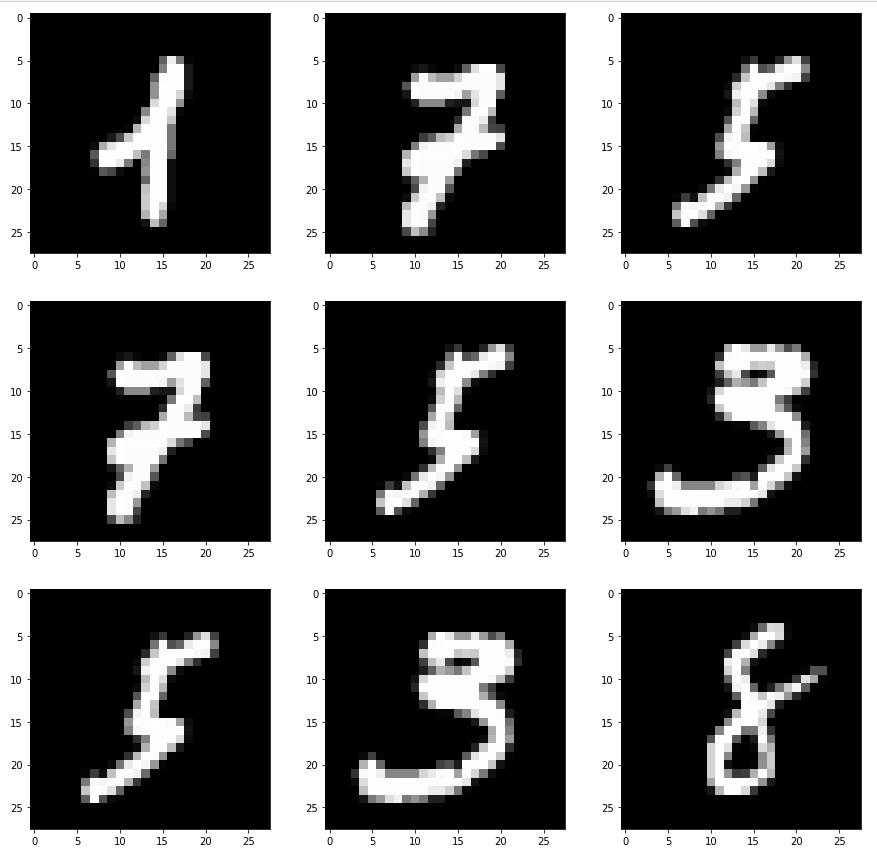
\includegraphics[width=1\linewidth]{img//intro/mnist.jpeg}
